\documentclass{article}

% packages
\usepackage{amsmath, amsthm, thmtools, amsfonts, amssymb, luacode, catchfile, tikzducks, hyperref, ifthen}
\ifcsname c@kobocompile\endcsname
	\usepackage[a5paper, total={1072pt, 1448pt}, margin=10pt, includeheadfoot]{geometry} % set page margins
\else
	\usepackage[a4paper, margin=50pt, includeheadfoot]{geometry}
\fi
\usepackage[shortlabels]{enumitem}
\usepackage[skip=3pt, indent=0pt]{parskip}

% language
\usepackage[bidi=basic, layout=tabular, provide=*]{babel}
\ifcsname c@english\endcsname
	\babelprovide[main, import]{english}
\else
	\babelprovide[main, import]{hebrew}
	\babelprovide{rl}
\fi
%\babelfont{rm}{Libertinus Serif}
\babelfont{rm}[Renderer=Harfbuzz]{Libertinus Serif}
\babelfont{sf}{Libertinus Sans}
\babelfont{tt}{Libertinus Mono}

% style
\AddToHook{cmd/section/before}{\clearpage}	% Add line break before section
\linespread{1.3}
\setcounter{secnumdepth}{0}		% Remove default number tags from sections, this won't do well with theorems
\AtBeginDocument{\setlength{\belowdisplayskip}{3pt}}
\AtBeginDocument{\setlength{\abovedisplayskip}{3pt}}
\graphicspath{ {../images/} }

% operators
\DeclareMathOperator\cis{cis}
\DeclareMathOperator\Sp{Sp}
\DeclareMathOperator\tr{tr}
\DeclareMathOperator\im{Im}
\DeclareMathOperator\re{Re}
\DeclareMathOperator\diag{diag}
\DeclareMathOperator*\lowlim{\underline{lim}}
\DeclareMathOperator*\uplim{\overline{lim}}
\DeclareMathOperator\rng{rng}
\DeclareMathOperator\Sym{Sym}
\DeclareMathOperator\Arg{Arg}
\DeclareMathOperator\Log{Log}
\DeclareMathOperator\dom{dom}
\DeclareMathOperator\supp{Supp}
\DeclareMathOperator\var{Var}
\DeclareMathOperator\cov{Cov}

% commands
%\renewcommand\qedsymbol{\textbf{מש''ל}}
%\renewcommand\qedsymbol{\fbox{\emoji{lizard}}}
\newcommand{\Aa}[0]{\mathcal{A}}
\newcommand{\Bb}[0]{\mathcal{B}}
\newcommand{\CC}[0]{\mathbb{C}}
\newcommand{\Cc}[0]{\mathcal{C}}
\newcommand{\EE}[0]{\mathbb{E}}
\newcommand{\FF}[0]{\mathbb{F}}
\newcommand{\Ff}[0]{\mathcal{F}}
\newcommand{\Ii}[0]{\mathcal{I}}
\newcommand{\Gg}[0]{\mathcal{G}}
\newcommand{\Ll}[0]{\mathcal{L}}
\newcommand{\Mm}[0]{\mathcal{M}}
\newcommand{\NN}[0]{\mathbb{N}}
\newcommand{\Nn}[0]{\mathcal{N}}
\newcommand{\PP}[0]{\mathbb{P}}
\newcommand{\Pp}[0]{\mathcal{P}}
\newcommand{\QQ}[0]{\mathbb{Q}}
\newcommand{\RR}[0]{\mathbb{R}}
\newcommand{\Rr}[0]{\mathcal{R}}
\newcommand{\Ss}[0]{\mathcal{S}}
\newcommand{\TT}[0]{\mathbb{T}}
\newcommand{\Uu}[0]{\mathcal{U}}
\newcommand{\Vv}[0]{\mathcal{V}}
\newcommand{\Ww}[0]{\mathcal{W}}
\newcommand{\ZZ}[0]{\mathbb{Z}}
\newcommand{\acts}[0]{\circlearrowright}
\newcommand{\explain}[2] {
	\begin{flalign*}
		 && \text{#2} && \text{#1}
	\end{flalign*}
}
\newcommand{\maketitleprint}[0]{ \begin{center}
	%\begin{tikzpicture}[scale=3]
	%	\duck[graduate=gray!20!black, tassel=red!70!black]
	%\end{tikzpicture}	
	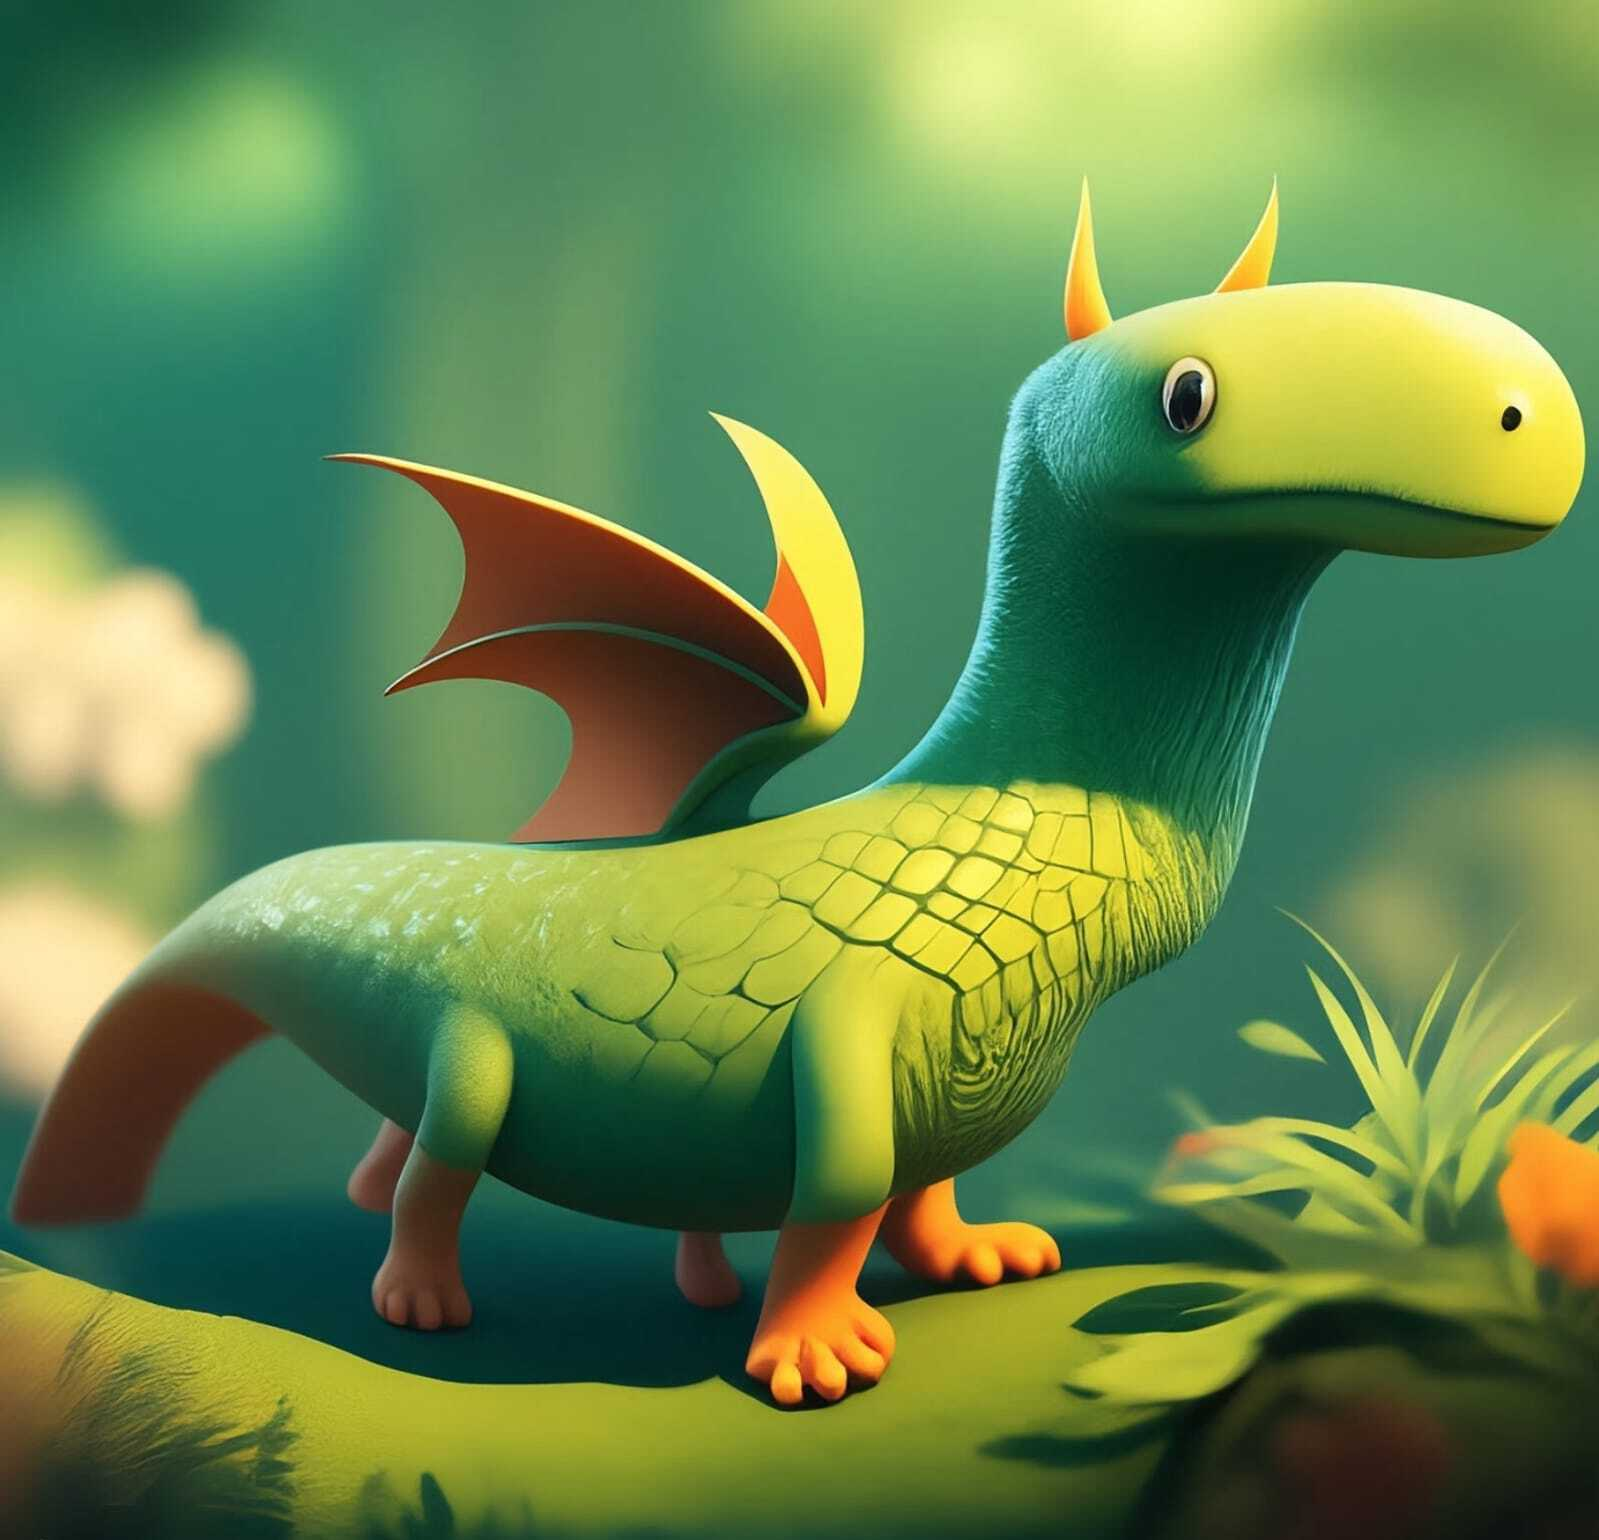
\includegraphics[width=6cm]{cover}
\end{center}
}

% theorem commands
\newtheoremstyle{c_remark}
	{}	% Space above
	{}	% Space below
	{}% Body font
	{}	% Indent amount
	{\bfseries}	% Theorem head font
	{}	% Punctuation after theorem head
	{.5em}	% Space after theorem head
	{\thmname{#1}\thmnumber{ #2}\thmnote{ \normalfont{\text{(#3)}}}}	% head content
\newtheoremstyle{c_definition}
	{3pt}	% Space above
	{3pt}	% Space below
	{}% Body font
	{}	% Indent amount
	{\bfseries}	% Theorem head font
	{}	% Punctuation after theorem head
	{.5em}	% Space after theorem head
	{\thmname{#1}\thmnumber{ #2}\thmnote{ \normalfont{\text{(#3)}}}}	% head content
\newtheoremstyle{c_plain}
	{3pt}	% Space above
	{3pt}	% Space below
	{\itshape}% Body font
	{}	% Indent amount
	{\bfseries}	% Theorem head font
	{}	% Punctuation after theorem head
	{.5em}	% Space after theorem head
	{\thmname{#1}\thmnumber{ #2}\thmnote{ \text{(#3)}}}	% head content

\ifcsname c@english\endcsname
	\theoremstyle{plain}
	\newtheorem{theorem}{Theorem}[section]
	\newtheorem{lemma}[theorem]{Lemma}
	\newtheorem{proposition}[theorem]{Proposition}
	\newtheorem*{proposition*}{Proposition}
	%\newtheorem{corollary}[theorem]{אין חלופה עברית}

	\theoremstyle{definition}
	\newtheorem{definition}[theorem]{Definition}
	\newtheorem*{definition*}{Definition}
	\newtheorem{example}{Example}[section]
	\newtheorem{exercise}{Exercise}[section]

	\theoremstyle{remark}
	\newtheorem*{remark}{Remark}
	\newtheorem*{solution}{Solution}
	\newtheorem{conclusion}[theorem]{Conclusion}
	\newtheorem{notation}[theorem]{Notation}
\else
	\theoremstyle{c_plain}
	\newtheorem{theorem}{משפט}[section]
	\newtheorem{lemma}[theorem]{למה}
	\newtheorem{proposition}[theorem]{טענה}
	\newtheorem*{proposition*}{טענה}
	%\newtheorem{corollary}[theorem]{אין חלופה עברית}

	\theoremstyle{c_definition}
	\newtheorem{definition}[theorem]{הגדרה}
	\newtheorem*{definition*}{הגדרה}
	\newtheorem{example}{דוגמה}[section]
	\newtheorem{exercise}{תרגיל}[section]

	\theoremstyle{c_remark}
	\newtheorem*{remark}{הערה}
	\newtheorem*{solution}{פתרון}
	\newtheorem{conclusion}[theorem]{מסקנה}
	\newtheorem{notation}[theorem]{סימון}
\fi

% Questions related commands
\newcounter{question}
\setcounter{question}{1}
\newcounter{sub_question}
\setcounter{sub_question}{1}

\ifcsname c@english\endcsname
	\newcommand{\question}[1][0]{
		\ifthenelse{#1 = 0}{}{\setcounter{question}{#1}}
		\section{Question \arabic{question}}
		\addtocounter{question}{1}
		\setcounter{sub_question}{1}
	}

	\newcommand{\subquestion}[1][0]{
		\ifthenelse{#1 = 0}{}{\setcounter{sub_question}{#1}}
		\subsection{Part \alph{sub_question}}
		\addtocounter{sub_question}{1}
	}
\else
	\newcommand{\question}[1][0]{
		\ifthenelse{#1 = 0}{}{\setcounter{question}{#1}}
		\section{שאלה \arabic{question}}
		\addtocounter{question}{1}
		\setcounter{sub_question}{1}
	}

	\newcommand{\subquestion}[1][0]{
		\ifthenelse{#1 = 0}{}{\setcounter{sub_question}{#1}}
		\subsection{סעיף \localecounter{letters.gershayim}{sub_question}}
		\addtocounter{sub_question}{1}
	}
\fi

% import lua and start of document
\directlua{common = require ('../common')}

\GetEnv{AUTHOR}

% headers
\author{\AUTHOR}
\date\today

\title{פתרון מטלה 13 --- מבוא ללוגיקה, 80423}

\begin{document}
\maketitle
\maketitleprint{}

\question{}
הוכחת משפט הרברן החלש.
תהי $L$ שפה לתחשיב יחסים עם סימן קבוע אחד לפחות, $\psi$ נוסחה חסרת כמתים עם משתנים חופשיים $x_0, \dots, x_{n - 1}$ ו־$\varphi = \forall x_0 \dots \forall x_{n - 1} \psi(x_0, \dots, x_{n - 1})$.
תהי $\Psi$ קבוצה סופית של פסוקים כוללים כך ש־$\Psi \cup \{ \varphi \}$ אינה עקבית.

\subquestion{}
נניח בשלילה ש־$\Sigma = \Psi \cup \{ \psi(t_0, \dots, t_{n - 1}) \mid t_i \in \operatorname{constterm}_L \}$ היא ספיקה.
יהי $\Aa \models \Sigma$,
נראה שקבוצת שמות העצם הקבועים $B = \{ t^\Aa \mid t \in \operatorname{constterm}_L \}$ היא תת־מודל של $\Aa$.
\begin{proof}
	מתרגיל 9.12 בסיכום נובע שעלינו להראות סגירות של $B$ לפונקציות $F^\Aa$ לכל סימן פונקציה של $L$, וכן $\forall c \in \operatorname{const}_L, c^\Aa \in B$.
	יהי $F \in \operatorname{Func}_{L, n}$ עבור $n < \omega$,
	אבל מהגדרת $\operatorname{constterm}_L$ נובע שאם $t_0, \dots, t_{n - 1} \in \operatorname{constterm}_L$ אז $F(t_0, \dots, t_{n - 1}) \in \operatorname{constterm}_L$ גם כן, ולכן $F^\Aa(t_0^\Aa, \dots, t_{n - 1}^\Aa) \in B$.
	בהתאם הקבוצה $B$ אכן סגורה לסימני פונקציה.
	נבחין כי מהגדרה גם אם $c \in \operatorname{const}_L$ אז $c \in \operatorname{constterm}_L$ ולכן $c^\Aa \in B$, ובהתאם מתקיים $\Bb \subseteq \Aa$ כפי שרצינו.
\end{proof}

\subquestion{}
נסיק ש־$\Bb \models \Sigma$.
\begin{proof}
	בתרגיל 7 שאלה 3 הוכחנו שאם $\Bb \subseteq \Aa$ וכן $\Aa \models \phi$ פסוק כולל, אז $\Bb \models \phi$.
	נבחין גם שאם $\phi \in \Sigma$ אז מהנתון הוא כולל, ולכן נסיק ש־$\Bb \models \Psi$.
	נבחין כי גם $\Bb \models \forall x_0, \dots, x_{n - 1} \psi(x_0, \dots, x_{n - 1}) \iff \forall x_0, \dots, x_{n - 1} \in B, \psi(x_0, \dots, x_{n - 1})$, כלומר הלוקאליזציה של $\psi$ ל־$\Bb$ היא פסוק כולל, ולכן גם מתקיים.
	נסיק ש־$\Bb \models \Sigma$.
\end{proof}

\subquestion{}
נסיק שמתקיים גם $\Bb \models \Psi \cup \{ \varphi \}$.
\begin{proof}
	למעשה כבר טענו בסעיף הקודם, $\varphi^B$ היא הפסוק $\forall x_0, \dots, x_{n - 1} \in \operatorname{constterm}_L, \psi(x_0, \dots, x_{n - 1})$, ולכן נובע מאבסולוטיות הטענה חלה.

	נפתור את הסעיף גם בחומר של הקורס.
	אנו כבר יודעים ש־$\Bb \models \Psi$, לכן מספיק להוכיח ש־$\Bb \models \varphi$.
	כמובן $\Bb \models \varphi \iff \forall x_0, \dots, x_{n - 1} \in B, \Bb \models \psi(x_0, \dots, x_{n - 1})$.
	אבל $x_0, \dots, x_{n - 1} \in B \iff x_0, \dots, x_{n - 1} \in \operatorname{constterm}_L$ ולכן $\psi(x_0, \dots, x_{n - 1}) \in \Sigma$ ובהתאם $\Aa \models \psi(x_0, \dots, x_{n - 1})$.
	נוכל להסיק שגם $\Bb \models \psi(x_0, \dots, x_{n - 1})$ ובהתאם נובע $\Bb \models \varphi$.
\end{proof}

\subquestion{}
נסיק שקיימת $\Sigma' \subseteq \Sigma$ סופית שאיננה עקבית.
\begin{proof}
	נוכל להסיק מהסעיפים הקודמים $\Sigma \models \varphi$, ולכן מנאותות גם $\Sigma \vdash \varphi$, נבחר קבוצה סופית של פסוקים $\Sigma' \subseteq \varphi$ כך שעדיין מתקיים $\Sigma' \vdash \varphi$.
	מהנתונים נובע גם $\Psi \models \lnot \varphi$ ולכן נרחיב את $\Sigma'$ להכיל את הפסוקים המעידים על כך (קבוצה סופית), ונקבל את המבוקש.
\end{proof}

\question{}
יהיו $\Aa_0 = \langle A_0, <_{A_0} \rangle, \Aa_1 = \langle A_1, <_{A_1} \rangle$ סדרים קוויים.
נגדיר $\Aa_0 + \Aa_1 = \langle A_0 \times \{ 0 \} \cup A_1 \times \{ 1 \}, <_{A_0 + A_1} \rangle$ כאשר $<_{A_0, A_1}$ מוגדר כסדר לקסיקוגרפי.

\subquestion{}
נראה שהסדר $<_{A_0 + A_1}$ הוא קווי.
\begin{proof}
	נסיק ישירות מפתרון מטלה 7 תרגיל 3 מתורת הקבוצות\footnote{ניתן לצפות בפתרון זה \href{https://raw.githubusercontent.com/D95-waka/Math/refs/heads/master/Set_Theory/bin/ex07.pdf}{כאן}}
\end{proof}

\subquestion{}
נראה שמתקיים $\langle \ZZ, < \rangle \equiv \langle \ZZ + \ZZ, < \rangle$ אבל $\langle \ZZ, < \rangle \not\cong \langle \ZZ + \ZZ, < \rangle$.
\begin{proof}
	נשתמש באסטרטגיה המתוארת ב־16.46 ללא שינויים כלל ונבחין כי הוכחתה עדיין תקפה.
	אם זאת שכן ניתן להסתכל על כל אחד מהסדרים הקוויים שקיבלנו כחיבור שני סדרים קוויים עם מינימום כך שאחד מהם התהפך וחובר לשני.
	נסיק אם כן ש־$\langle \ZZ, < \rangle \equiv \langle \ZZ + \ZZ, < \rangle$.
	מהצד השני, אילו קיים $f$ איזומורפיזם המעיד על $\langle \ZZ, < \rangle \cong \langle \ZZ + \ZZ, < \rangle$, אז אם $f(x) = \langle x', d \rangle$ אז נובע שלכל $y \in \ZZ$, גם $f(x + y) = \langle x' + y, d \rangle$.
	בהתאם נסיק שאין מקור ל־$\langle 0, 1 - d \rangle$ ונקבל סתירה להיות $f$ על, לכן נסיק ש־$\langle \ZZ, < \rangle \not\cong \langle \ZZ + \ZZ, < \rangle$
\end{proof}

\subquestion{}
נכתוב אקסיומות לתורה השלמה $\langle \ZZ, < \rangle$.
\begin{proof}
	תהי $T_0$ תורת הסדרים הקוויים, אז נגדיר
	\[
		T = T_0 \cup \{
			\forall x \exists y (\forall z, (x < z \rightarrow x < y < z)), 
			\forall x \exists y (\forall z, (z < x \rightarrow z < y < x))
		\}
	\]
	תורה המתארת סדר קווי כך שלכל איבר יש עוקב מיידי וקודם מיידי.

	נבחין כי אם $\Mm \models T$ אז $|M| = \omega$, זאת שכן לא יתכן שהמודל יהיה סופי, ועל־ידי איזומורפיזם סדרים של תורת הקבוצות נסיק שלא יתכן ש־$|M| > \omega$.
	נבחין ש־$\Mm \cong \ZZ^n$ עבור $n < \omega$.
	זאת נוכל להוכיח על־ידי מציאת החזקה המינימלית בה יש שיכון.
	על־ידי הרחבת טענת סעיף ב' באינדוקציה נסיק ש־$\Mm \equiv \langle \ZZ, < \rangle$, ולכן $T$ היא $\aleph_0$־קטגורית ובפרט שלמה.
\end{proof}

\question[4]{}
נגדיר $L = L_{\text{fields}} \cup \{ P \}$ עבור $P$ סימן יחס חד־מקומי.
נסמן ב־$T$ את התורה המכילה קומוטטיביות, אסוציאטיביות וקיום איבר נייטלי לחיבור וכפל, פילוג ואת הכללים,
\begin{enumerate}
	\item $P(0)$
	\item $\forall x, P(X) \rightarrow P(x + 1)$
	\item $0 \ne 1$
\end{enumerate}
עוד נגדיר שמות עצם $\langle e_n \mid n < \omega \rangle$ על־ידי
\[
	e_n
	= \begin{cases}
		1 + 1 & n = 0 \\
		e_n \cdot e_n & \text{else}
	\end{cases}
\]

\subquestion{}
נוכיח שמתקיים $T \vdash P(e_{10})$.
\begin{proof}
	נניח ש־$\Mm \models T$, לכן $\Mm$ ללא $P$ הוא שדה.
	נוכיח באינדוקציה ש־$\Mm \models P(n)$ לכל $n \in \{0, 1, 1 + 1, \dots \}$.
	נתון כי $\Mm \models 0$, זהו בסיס האינדוקציה.
	נניח ש־$\Mm \models P(n)$ ונבחן את $P(n + 1)$, מתקיים $\Mm \models P(n), P(n) \rightarrow P(n + 1)$ ולכן ממודוס־פוננס גם $\Mm \models P(n + 1)$.

	נבחין גם ש־$e_{10}^\Mm = 1 + 1 + \cdots + 1$, זאת שכן מחוקי פילוג וניטרליות הכפל נובע $e_{10}^\Mm = {(1 \cdot e_{10})}^\Mm = {(1 + \cdots + 1)}^\Mm$, לכן נובע גם $\Mm \models P(e_{10})$.
	
	מצאנו כי כל מודל $\Mm \in \operatorname{Mod}(T)$ מקיים $\Mm \models P(e_{10})$ ולכן $T \models P(e_{10})$ וממשפט השלמות $T \vdash P(e_{10})$.
\end{proof}

\subquestion{}
נתאר עץ היסק ל־$T \vdash P(e_{10})$ כך שיש בו עשרות קודקודים בלבד.
\begin{solution}
	נגדיר $\varphi(y) = \forall x (P(x) \rightarrow P(x + y))$, ונבחין כי נתון $\varphi(y) \in T$ (מתלכד עם פסוק נתון), וכן נבחין ש־$\varphi(n), \varphi(m) \vdash \varphi(n + m)$, נבנה עץ היסק,
	\begin{enumerate}
		\item $\lnot \varphi(n + m)$
		\item $\lnot (P(c) \to P(c + n + m))$, הוספת עד
		\item $P(c)$, כללי גרירה
		\item $\lnot P(c + n + m)$, כללי גרירה
		\item $\varphi(n)$, הוספת הנחה
		\item $\lnot \varphi(c + n)$, כללי גרירה
		\item $\varphi(m)$, הוספת הנחה
		\item $\varphi(c + n + m)$, כללי גרירה, וסתירה
	\end{enumerate}
	לכן בפרט $\varphi(n) \vdash \varphi(2n)$ בכמות קטנה (נוכל לעשות זאת עם שישה קודקודים בלבד), נוכל אם כן לקבל את $T \vdash \varphi(2)$ ואת $\varphi(2) \vdash \varphi(4)$ וכן הלאה $n$ פעמים בכמות קטנה של קודקודים בכל פעם.
	בהתאם נקבל לאחר $2^{10}$ מהלכים כאלה גם את $T \vdash \varphi(e_{10})$, כאשר לעץ זה יהיו סדר גודל של אלפי קודקודים בלבד (למעשה כ־6000).

	נגדיר $\psi(y) = \forall x (P(x) \rightarrow P(x \cdot y))$, נבחין כי $\psi(n), \psi(m) \vdash \psi(nm)$ בשישה קודקודים באופן דומה.
	נבחן את $\psi$ עם הגבלה, כלומר $\psi'(y) = \forall x (x \in \{ d_n \mid n < 10 \}) \rightarrow (P(x) \rightarrow P(x \cdot y))$, כאשר,
	\[
		d_n
		= \begin{cases}
			1 + 1 & n = 0 \\
			d_{n - 1} + d_{n - 1} & n > 0
		\end{cases}
	\]
	נבחין כי את $T \vdash \psi'(2)$ אנו יכולים להוכיח די בקלות עם עץ ההיסק הבא,
	\begin{enumerate}
		\item $\lnot \psi'(2)$
		\item $c \in \{ d_n \mid n < 10 \}$, $P(c)$, $P(c + c)$, הוספת עד
		\item $c = d_{10}$, הנחה שאיננה בהכרח נכונה, אך הנחה זו תגרור את עץ ההיסק הארוך ביותר, לכן נניח אותה
		\item $\varphi(d_{9})$, הדבקת עץ ההיסק הרלוונטי
		\item $P(d_{10})$, שימוש בכללי ההיסק, וסתירה
	\end{enumerate}
\end{solution}

\end{document}
